\chapter{Introduction}
\label{chap:intro}
\graphicspath{{Introduction/Images/}}

At the dawn of the nineteenth century, Italian astronomer Giuseppe Piazzi was engrossed in observing the Taurus constellation to update a star catalog. On January 1 1801, atop the Palermo observatory in Sicily, he observed a light which was not mentioned in the catalog. He followed the strange light for a few more nights, eventually realizing that he had discovered a small planet between Mars and Jupiter. He named the minor planet Ceres and it became the first of its kind to be discovered by humans. Broadly speaking, it became the first asteroid to ever be discovered \parencite{cunningham2016discovery}. Soon after this discovery, three other minor planets were discovered in the gap between Mars and Jupiter. Pallas was discovered in 1802, followed by Juno in 1804, and finally Vesta in 1807. After the discovery of Ceres and Pallas, renowned astronomer William Herschel realized that these are a new species of celestial bodies and proposed to call them asteroids (which in Greek means star-like) instead of minor planets. For nearly 40 years after the discovery of Vesta, no additional discoveries were made. Then once again in the second half of the nineteenth century, astronomers started discovering more and more asteroids until they realized that there is a whole belt of it between Mars and Jupiter \parencite{bottke2002asteroids}.
%
\newline\newline
%
Asteroids are rocky, airless celestial bodies in our Solar System that orbit the Sun and are quite small in size compared to the planets. They can be viewed as remnants of the processes that formed the inner planets of our Solar System \parencite{nasa_asteroids_web}. Asteroids are mostly irregularly shaped with a few exceptions, like Ceres, that have a nearly spherical shape. \Cref{fig:asteroid_shapes} provides a view on the different morphologies of asteroids \parencite{nasa_asteroids_web}. They are typically categorized based on their location in the Solar System. A large number of asteroids are found in the region between Mars and Jupiter and are called as \glspl{MBO}. A relatively smaller number of asteroids, called \glspl{NEA}, have orbits that are very close to and/or crosses the heliocentric orbit of Earth. Asteroids at the $L_4$ and $L_5$ Lagrange points of Jupiter, sharing its orbit around the Sun, are termed as Trojans. Then we have Centaurs, asteroids whose orbit lies between or crosses that of the Giant planets in our Solar System. The fifth and the final category is that of the \glspl{TNO} i.e. asteroids with orbit beyond that of Neptune and reaching as far as the Oort cloud \parencite{planetarySciencePater}. The distribution of asteroids in the inner and outer Solar System is shown in \Cref{fig:asteroid_distribution}.
% Asteroids are rocky, airless celestial bodies in our Solar System that orbit the Sun and are found in quite large numbers. Relative to the planets, these asteroids are very small and are sometimes even referred to as minor planets. They can be viewed as remnants of the processes that formed the planets of the inner Solar System. Asteroids come in different shapes and sizes, and while most are irregularly shaped, a few are found to be nearly spherical. \Cref{fig:asteroid_shapes} provides a view on the different morphologies of asteroids \parencite{nasa_asteroids_web}. They are typically classified based on their location in our Solar System. A large number of asteroids are found in the region between Mars and Jupiter, called the \gls{MAB}, and these asteroids are hence called as the \gl{MBO}}. A rather smaller number of objects whose orbit lies close to that of Earth or crosses the Earth's orbit itself are termed as \gl{NEO}}. Next, sharing Jupiter's orbit around its $L_4$ and $L_5$ Lagrange points are the \texti{Trojan} asteroids, and the ones whose orbit lies between or crosses that of the giant planets (Jupiter, Saturn, Uranus, Neptune) in our Solar System are called the \texti{Centaurs}. The vast majority of small bodies in our Solar System have orbits that extend beyond that of Neptune and are termed as \gls{TNO}}. These are further classified into \gls{CKBO}, objects with low eccentric orbits resonant with Neptune, and \gls{SDO}, objects with highly eccentric and non-resonating orbits. There are small bodies even beyond the \gls{TNO}s and are found in a very distant region called the \texti{Oort Cloud} \parencite{planetarySciencePater}. The distribution of asteroids in the inner and outer Solar system is shown in \Cref{fig:asteroid_distribution}.
%%%
\begin{figure}[htb]
\centering
\captionsetup{justification=centering}
    \begin{minipage}{0.48\columnwidth}
        \subfloat[]{
            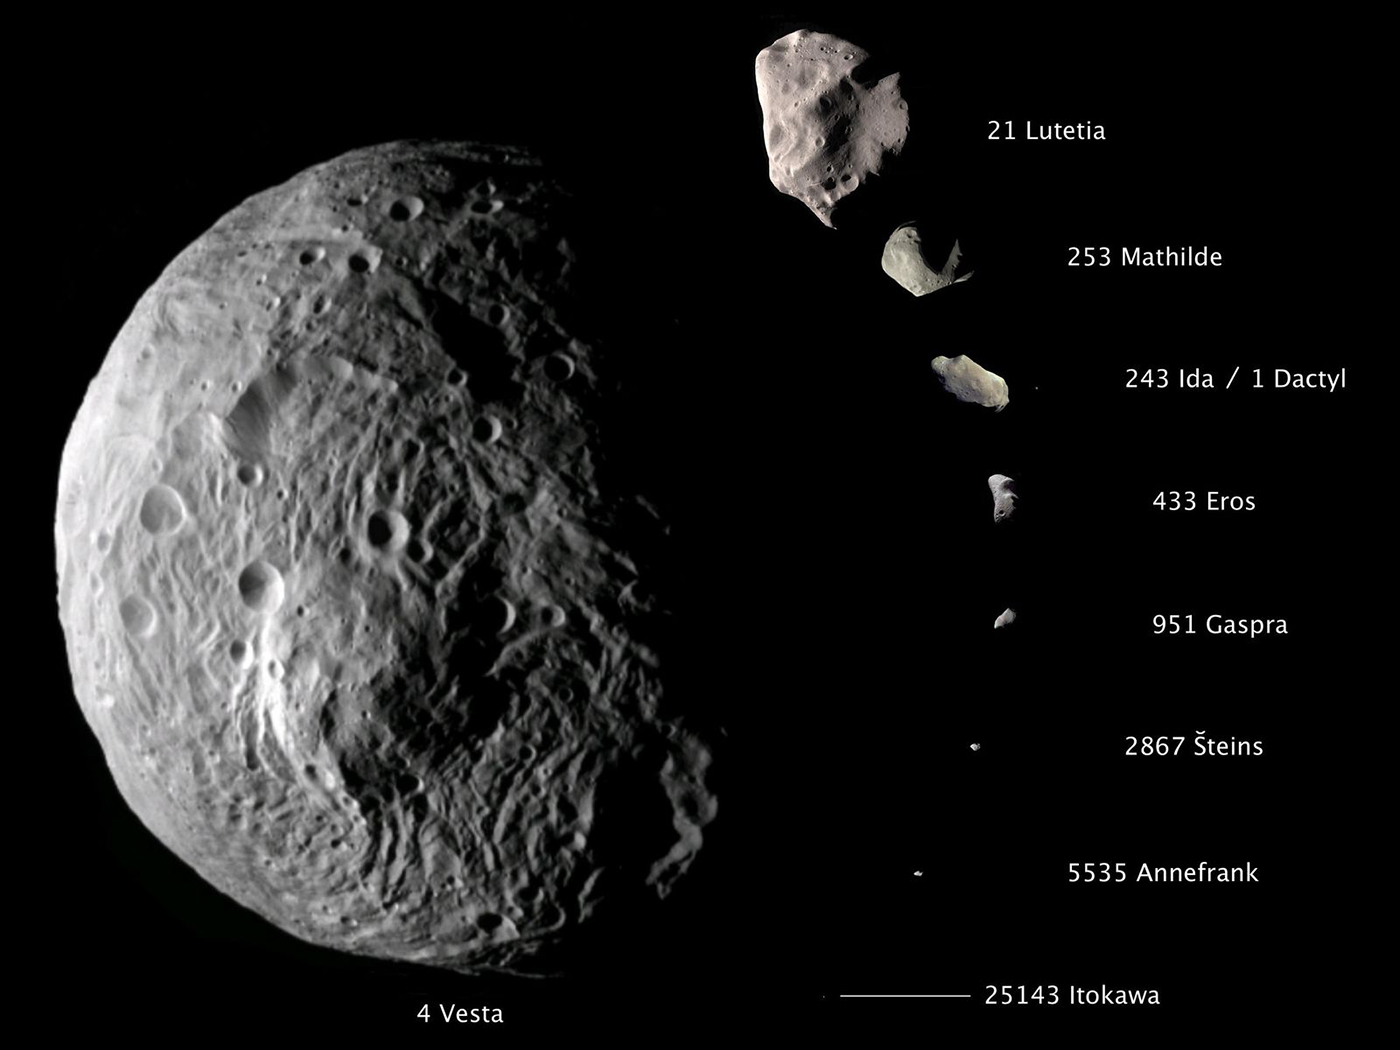
\includegraphics[width=\columnwidth, height=0.5\textheight, keepaspectratio=true]{asteroid_size_comparison.jpg}
            \label{fig:vesta_compared_with_other_asteroids}
        }
    \end{minipage}
    \begin{minipage}{0.48\columnwidth}
        \subfloat[]{
            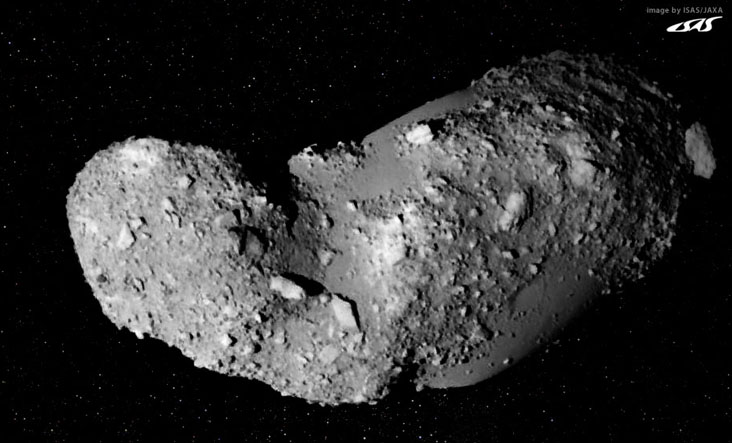
\includegraphics[width=\columnwidth, height=0.25\textheight, keepaspectratio=true]{itokawa.jpg}
            \label{fig:itokawa_image}
        }
        \\[3mm]
        \subfloat[]{
            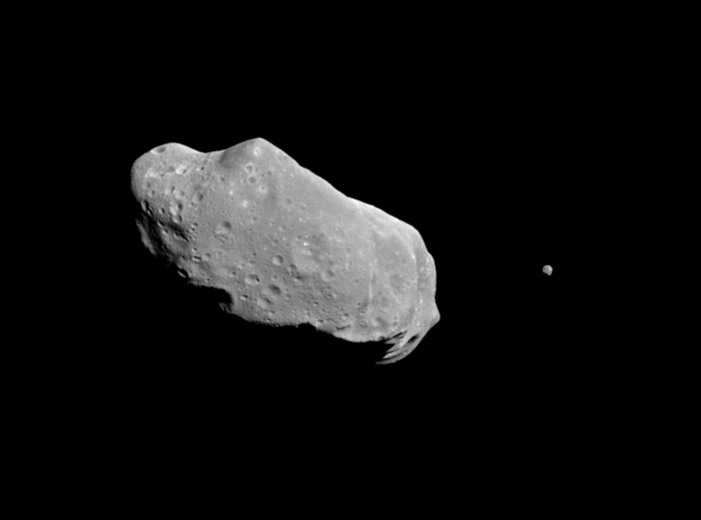
\includegraphics[width=\columnwidth, height=0.25\textheight, keepaspectratio=true]{Ida_Dactyl.jpg}
            \label{fig:ida_dactyl_image}
        }
    \end{minipage}
\caption{Satellite imagery depicting different morphologies of asteroids. \protect\subref{fig:vesta_compared_with_other_asteroids} Size and shape variations amongst a few known asteroids, \protect\subref{fig:itokawa_image} Asteroid Itokawa with its rocky and rough surface, \protect\subref{fig:ida_dactyl_image} Asteroid Ida with its moon Dactyl orbiting around it \parencite{nasa_asteroids_web}.}
\label{fig:asteroid_shapes}
\end{figure}
\FloatBarrier
%%%
Due to their extremely small sizes, asteroids can not have high internal pressures and temperatures, which means that they could have potentially preserved the early chemistry of our Solar System \parencite{hayabusaTouchdownDynamics}. This makes them a valuable source for us to learn about the history and origin of our Solar System. It is hypothesized that during the early years of Earth's formation, carbon-based molecules and other volatile materials which serve as the basic building-blocks of life, could have been delivered to Earth through asteroid impacts \parencite{jpl_asteroid_web}. Finally, some asteroid types are rich in resources and contain vast supplies of precious metals \parencite{asteroidPreciousMetalSource} and water \parencite{asteroidWaterSource}, which could potentially be mined and used to aid further exploration and colonization of our Solar System \parencite{jpl_asteroid_web}. Thus in light of this, asteroid exploration, both in-situ and ex-situ, has gained significant importance not only among the scientific community but among the private space industry as well, with more and more future missions being planned to these small bodies. The \gls{NEAR} spacecraft launched by the \gls{NASA} in 1996, as part of their Discovery program, became the first spacecraft in history to orbit an asteroid (433 Eros) and eventually land on it. The spacecraft spent almost a year around Eros, providing extended and comprehensive observations of surface morphology, shape, internal structure and physical properties of the asteroid \parencite{nearMission}. The Hayabusa mission (formerly MUSES-C) by the \gls{JAXA} entered into orbit around asteroid Itokawa in 2005 and became the first mission to sample the surface of an asteroid, which was subsequently returned to Earth for analysis in 2010 \parencite{yanoHayabusaTouchdown}. These missions have substantially increased our knowledge about the small bodies in our Solar System.
%
\newline\newline
%
%%%
\begin{figure}[htb]
\centering
\captionsetup{justification=centering}
    \subfloat[]{
        \fbox{
        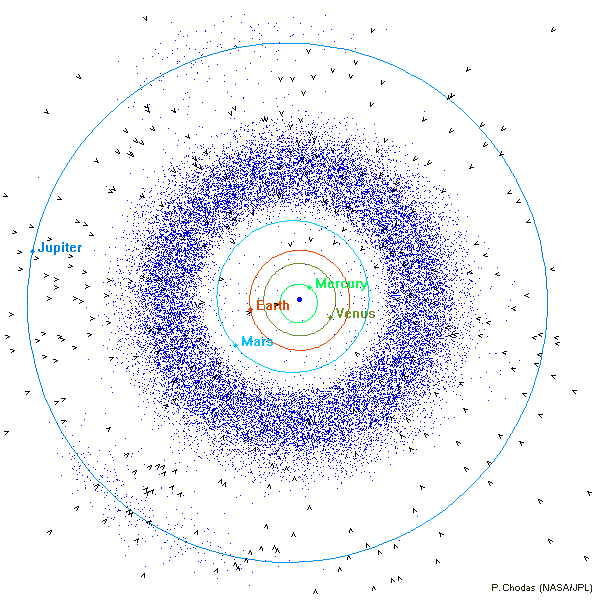
\includegraphics[width=0.5\linewidth, height=\textheight, keepaspectratio=true]{asteroid_distribution_orbit_plot_inverted.png}
        \label{fig:inner_asteroids}
        }
    }
    \subfloat[]{
        \fbox{
        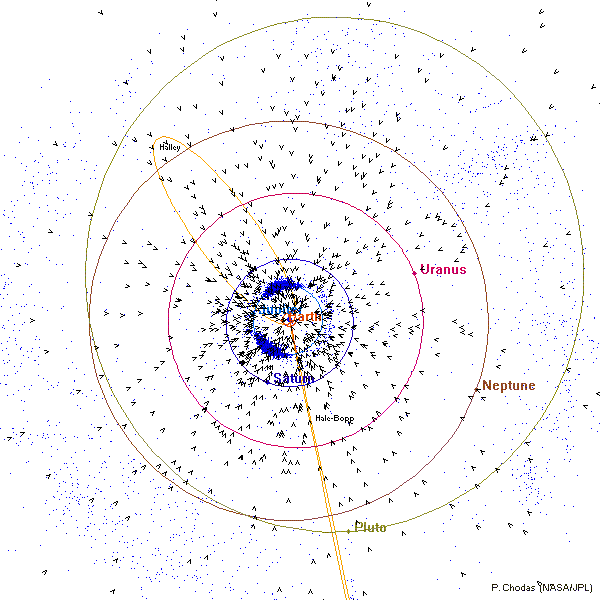
\includegraphics[width=0.5\linewidth, height=\textheight, keepaspectratio=true]{asteroid_distribution_outer_orbit_plot_inverted.png}
        \label{fig:outer_asteroids}
        }
    }
\caption{Distribution of asteroids in \protect\subref{fig:inner_asteroids} inner Solar System and \protect\subref{fig:outer_asteroids} outer Solar System. Asteroid locations are shown by blue-colored dots whereas the black-colored wedges pointing towards the Sun represent the comets. The diagrams are based on the small-bodies cataloged up until November 2016 \parencite{jpl_asteroid_web}. These images are color-inverted versions of the original.}
\label{fig:asteroid_distribution}
\end{figure}
\FloatBarrier
%%%
Two more asteroid rendezvous missions launched quite recently are of particular interest to this thesis. Following the success of Hayabusa, \gls{JAXA} launched another sample return mission called Hayabusa-2 to asteroid 1999 JU3, scheduled to be in orbit around it by mid-2018. It will perform a 1.5 year long close-proximity operation at the asteroid that includes surface sample acquisition, which will eventually be returned to Earth in a capsule, and a \SI{2}{\metre} wide cratering event to observe the sub-surface \parencite{TsudaHayabusa2SystemDesign}. The \gls{OSIRIS-REx} mission by \gls{NASA}, directed towards asteroid Bennu and scheduled to enter into an orbit around it in late 2018, will also retrieve a surface sample and return it back to Earth. It will employ a \gls{TAG} maneuver to acquire a sample within a 1.5 month long scheduled sampling period \parencite{berry2013osiris}. Both missions are aiming to find out if organic material, volatiles and water itself were brought to Earth by such asteroids. These missions employ techniques for sample acquisition that could potentially disturb the state of regolith on the surface of the asteroid and loft it into an orbit. Even without any spacecraft interaction, material can be lofted from the surface of an asteroid due to meteoroid impacts. In either case, it is imperative to understand the complex dynamical environment around asteroids, not only for spacecraft operations and safety, but also to learn about the orbital motion of lofted regolith and its eventual fate. \gls{NASA} has identified the acquisition of such information as a \gls{SKG} for \glspl{NEO}, specifically article III-A-1: Expected particulate environment due to impact ejecta in \cite{nasa_skg}.
%
\newline\newline
%
The study of lofted regolith around an asteroid is by no means a new research topic. In the studies done previously \parencite{richter1995stability,lee1996dust,scheeres1996orbits,scheeres2000ejecta,korycansky2004_impactEjecta,yarnoz2014passive}, we have witnessed certain minor drawbacks such as not always accounting for gravity and Solar perturbations together, or using an approximated analytical method to understand the dynamical environment that falls short on obtaining the entire spectra of initial conditions that could lead to different final outcomes (re-impact, escape or temporary capture) for lofted regolith, or not considering different size and density for the lofted regolith, and finally not considering the local direction with respect to a rotating asteroid in which the regolith is ejected. This thesis, thus, aims to include all of these shortfalls in a single study, and by using numerical simulation techniques, to add more fidelity in understanding what happens to regolith when it is lofted from the surface of an asteroid.
%
\newline\newline
%
The study of orbiting regolith is important for understanding the displacement of material on surface of the asteroid in case of natural or spacecraft-induced impact cratering events. From a mission design point-of-view, the ejecta from an impact cratering event could pose a serious threat to spacecraft and/or its instruments. By knowing the orbital behavior of regolith in advance, mission designers can make informed decisions on the trajectory design of spacecraft to avoid or reduce failure scenarios. Another important benefit that comes from a study like this is in the field of asteroid mining, whereby the regolith's orbital motion and final fate can be exploited to sort different materials in real time. The results from this thesis will thus aid mission designers in planning future asteroid missions and in answering the following research question:
\vspace{5mm}
%%%
\begin{center}
    \fbox{\parbox{0.8\textwidth}{
    \centering
    \textbf{\textit{Can we explain the orbital behavior and eventual fate of lofted regolith around an asteroid in presence of gravity and Solar perturbations?}}}
    }
\end{center}
%%%
\vspace{5mm}
The structure of this report is mentioned as follows: \Cref{chap:heritage} briefly discusses the past and the future missions to asteroids in the context of this thesis, and a few research publications that are relevant for our work. This paves the way to define the research questions and goals in \Cref{chap:research_questions}. \Cref{chap:dynamics_modeling} discusses the models for simulating an asteroid's gravity and the Solar perturbations, equations of motion for the regolith and its launch conditions, and finally a non-conservative algorithm to determine a regolith's guaranteed escape speed. The verification and validation of the simulation models can be found in \Cref{chap:v_and_v}. \Cref{chap:nonconservative} discusses the performance of the conservative guaranteed escape speed algorithm for a spherical and an ellipsoidal asteroid and the performance of the non-conservative algorithm for the ellipsoidal asteroid. \Cref{chap:dynamics_without_solar_perturbations} discusses the general characteristics of lofted regolith and its final fate for an ellipsoidal asteroid in the absence of Solar perturbations. \Cref{chap:dynamics_with_solar_perturbations} does the same analysis but in the presence of Solar perturbations and for regoliths of different size and density. \Cref{chap:conclusions} summarizes all the results by presenting answers to all the sub-research questions from \Cref{chap:research_questions}. Finally, \Cref{chap:recommendations} provides some recommendations for future work on our research topic.

% Asteroids are not only found as single, isolated bodies in the Solar System, but also as multi-body local systems consisting of two or three asteroids. Over 190 multiple asteroid systems have so far been detected in the Solar System. They are significantly diverse in terms of the size ratios of the individual asteroids, their orbit motion and separation around each other, implicating that the individual asteroids evolved differently over time \parencite{multipleAsteroids}. If two or three asteroids are bound to each other gravitationally, then they are termed as \textit{binary asteroids} and \textit{triple asteroids} respectively. An example of a binary asteroid system is shown in \Cref{fig:ida_dactyl_image}. However, if individual asteroids share similar heliocentric orbits but are not gravitationally bound to each other, then they are termed as \textit{asteroid pairs}. Within a pair, if the larger asteroid is itself a binary or a triple asteroid system, then the pair is termed as \textit{paired binary} or \textit{paired triple} respectively \parencite{multipleAsteroidsTerminology}. Asteroids can further be classified into categories based on their dimensions and thermal properties, and is discussed in \cite{multipleAsteroids}.
